% appendix.tex
\appendix

\section{Appendix A}


\label{appendix:gradient_fields}
\subsection{Interpreting The Gradient Fields}
\label{sec:interpret_gradient_fields}
The gradient descent field contains information about the loss landscape and the update path from the initial point. We chose 2 parameters for each program, corresponding to the 2 dimensions in the gradient fields. For \BPNoise, the x-axis is the HP cutoff and the y axis is the LP cut off. The values for the parameters are normalized from -1 to 1. In \BPNoise{} for example, the possible values for LP cut are defined in the \texttt{hslider} function in the range of 50 Hz-1000 Hz. The initial point is 100 Hz, which is normalized to around -0.95, as shown in the graph. The initial HP cutoff is set at 20, which normalizes to around -0.75 in the range of 1 Hz - 120 Hz.

The initial and target parameters are shown with green circle \greencircle~and star \greenstar~respectively. Each circle in the connected red circles \redcircles~ corresponds to an update to the initial values. The ideal successful experiment would entail a series of red dots connecting the initial values to the target values, meaning that each update step took the initial parameter values closer to the target. The background of the gradient field is a heatmap based on the value of the loss. The highest loss corresponds to a darker color, and the lowest loss---which should be around the target value---should be the white. 

The arrow in the middle of each heatmap square corresponds to the direction and magnitude of the gradients. The gradients here can be extremely large; signal processing functions can be unpredictable, and the gradients are calculated backwards sequentially through the signal processing chain, resembling similar calculations---associated with exploding gradients---in recurrent neural networks~\cite{gers2000learning}. For this reason gradient clipping is applied~\cite{goodfellow2016deep}.


\subsection{\BPNoise}
In \BPNoise, a noise signal is fed through a band-pass (BP) filter, which removes the frequencies between the low-pass (LP) and high-pass (HP) cutoff. As shown in Listing~\ref{lst:program0}, the target (or \texttt{true\_params}) is the HP of 100, and LP of 900, and the initial parameters are 20 and 100 respectively. 

Figure~\ref{fig:p0_losses} depicts the learning trajectory for all loss functions. Changes in filter cut-offs is mainly reflected in the frequency content of the sound.  All loss functions except for DTW-Onset are successful in finding the target. These results make intuitive sense, as the DTW-Onset loss primarily works by matching amplitude envelopes, yet the other loss functions primarily measure changes in frequency content. 

The heatmaps of L1-Spec, SIMSE-Spec, and JTFS also show low loss values closer to the target, unlike the DTW-Onset function.  

\subsection{\AddSineSaw}
\AddSineSaw{} is an additive program that combines a saw and a sine wave function (each with a different frequency) to create the output. The initial values for the frequencies being 800 Hz and 300 Hz, and the target of 200 Hz and 100 Hz. 

As show in Figure~\ref{sec:program1}, the Spectrogram losses quickly fail this test. The loss heatmaps here look reasonable, yet most gradients point to the wrong direction, and the iterative update steps quickly fall outside the parameter range as defined by the code, which makes recovery impossible. The DTW-Onset loss also fails to find the target, but gets close to the correct Saw frequency. What is notable here is that for the 3 failed loss functions, their gradient field indicates that the Sine Frequency (the vertical y-axis features) is not considered an important parameter, as most of the gradients do not have a strong vertical direction. We can speculate that this is due to the strong harmonic content of the saw wave relative to the sine waves.

A notable characteristic of the heatmaps is the diagonal line where the sine and saw frequencies are equal. All points on this line are outliers relative to their neighbouring points. This is because of the harmonic overlap where the sine frequency falls directly on top of the fundamental frequency of the saw wave. 

\subsection{\AmpMod}
Matching the dynamic amplitude change in the sound caused by the Sine oscillator is the main challange of this program, and we see that DTW-Onset loss is the only function successful at this task. JTFS and L1-Spectrogram loss find a value close to the true \textit{amp}, yet do not move towards the correct \textit{carrier} value. The DTW-Onset heatmap also shows reasonable gradients and loss-values corresponding to distance from the target. 

\subsection{\FMMod}
All loss functions except DTW-Onset perform poorly and fall outside the acceptable range within a few updates. DTW-Onset appears as the only promising function here. This loss crosses the correct amplitude modulation frequency, but fails to converge to the correct carrier frequency. 

In the DTW-Onset heatmap we see little change in loss values in the vertical plane corresponding to the carrier, however, the amplitude dimension has the minimal loss value around the target parameter. This again shows that the DTW-Onset loss excels at matching sound envelopes (or changes in sound volume over time) but is insensitive to frequency content. 
\begin{figure*}[htbp]
    \centering
    % Top row
    \begin{subfigure}[b]{0.49\textwidth}
        \centering
        \adjustbox{valign=t}{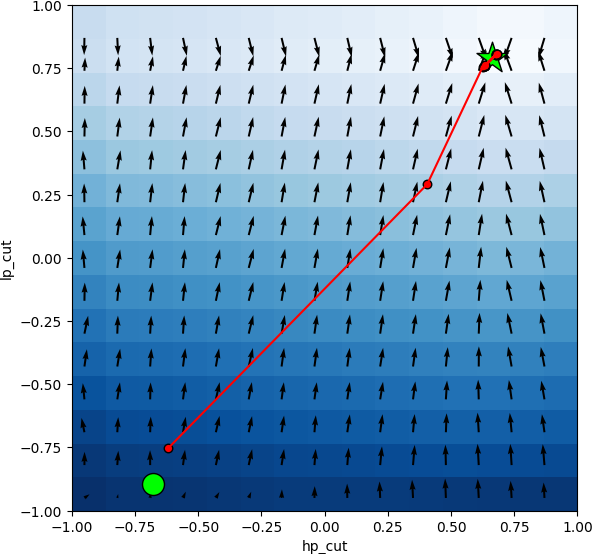
\includegraphics[width=\textwidth]{images/experiment_plots/p0_L1_Spec.png}}
        \caption{L1 spectrogram loss}
        \label{fig:p0_spec}
    \end{subfigure}
    \hfill
    \begin{subfigure}[b]{0.49\textwidth}
        \centering
        \adjustbox{valign=t}{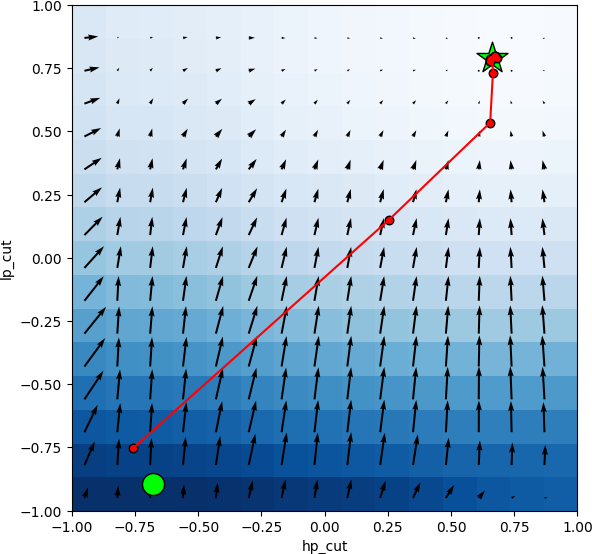
\includegraphics[width=\textwidth]{images/experiment_plots/p0_SIMSE_Spec.png}}
        \caption{SIMSE spectrogram loss}
        \label{fig:p0_simse}
    \end{subfigure}
    \vspace{0.5cm} 
    % Bottom row
    \begin{subfigure}[b]{0.49\textwidth}
        \centering
        \adjustbox{valign=t}{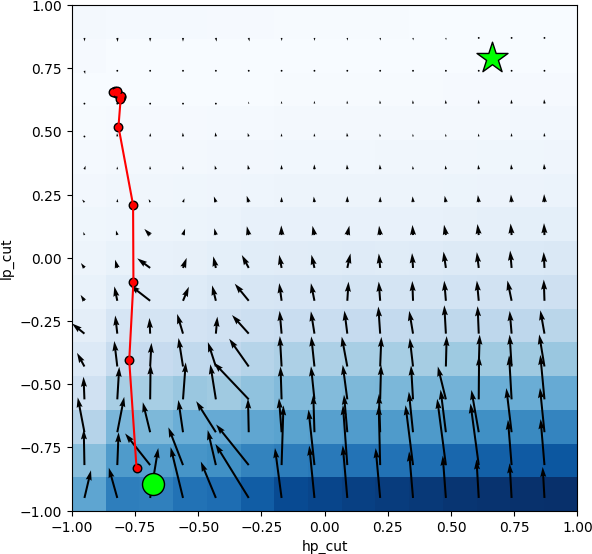
\includegraphics[width=\textwidth]{images/experiment_plots/p0_DTW_Onset.png}}
        \caption{DTW onset loss.}
        \label{fig:p0_dtw}
    \end{subfigure}
    \hfill
    \begin{subfigure}[b]{0.49\textwidth}
        \centering
        \adjustbox{valign=t}{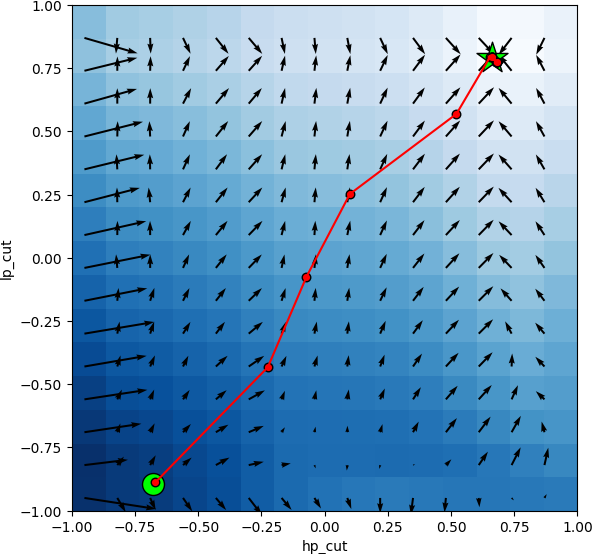
\includegraphics[width=\textwidth]{images/experiment_plots/p0_JTFS.png}}
        \caption{JTFS loss}
        \label{fig:p0_jtfs}
    \end{subfigure}

    \caption{Gradient descent fields for each loss with respect to \BPNoise. The initial and target parameters are shown with green circle \greencircle~and star \greenstar~respectively. High loss corresponds to dark-blue and low corresponds to white.}
    \label{fig:p0_losses}
\end{figure*}

\begin{figure*}[htbp]
    \centering
    % Top row
    \begin{subfigure}[b]{0.49\textwidth}
        \centering
        \adjustbox{valign=t}{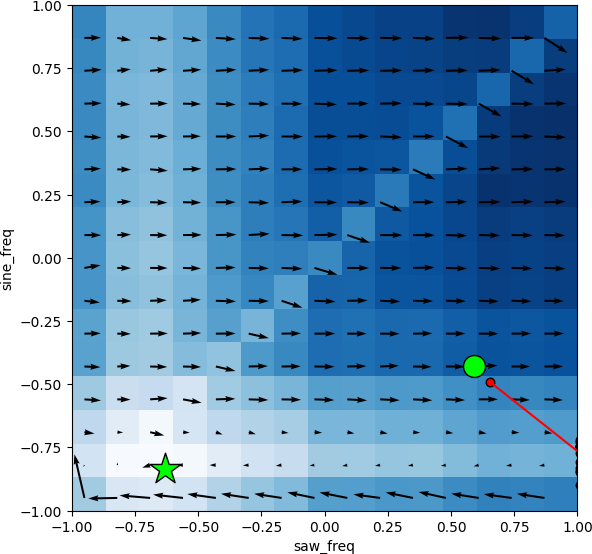
\includegraphics[width=\textwidth]{images/experiment_plots/p1_L1_Spec.png}}
        \caption{L1 spectrogram loss}
        \label{fig:p1_spec}
    \end{subfigure}
    \hfill
    \begin{subfigure}[b]{0.49\textwidth}
        \centering
        \adjustbox{valign=t}{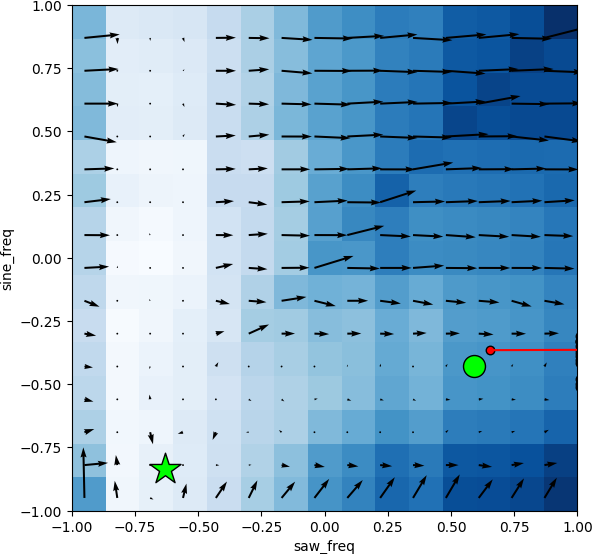
\includegraphics[width=\textwidth]{images/experiment_plots/p1_SIMSE_Spec.png}}
        \caption{SIMSE spectrogram loss}
        \label{fig:p1_simse}
    \end{subfigure}
    \vspace{0.5cm} 
    % Bottom row
    \begin{subfigure}[b]{0.49\textwidth}
        \centering
        \adjustbox{valign=t}{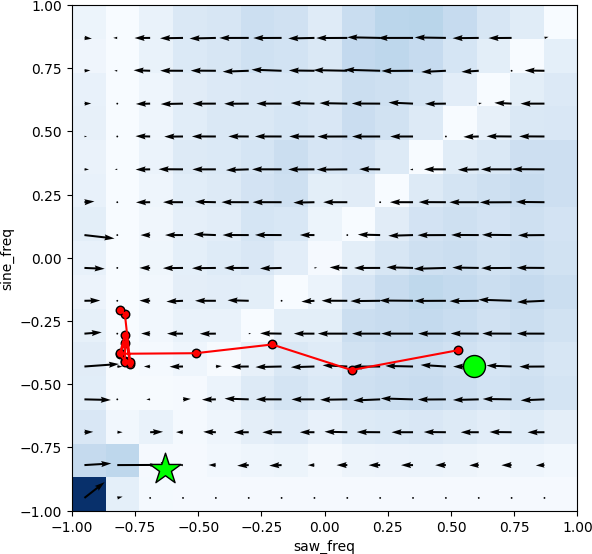
\includegraphics[width=\textwidth]{images/experiment_plots/p1_DTW_Onset.png}}
        \caption{DTW onset loss.}
        \label{fig:p1_dtw}
    \end{subfigure}
    \hfill
    \begin{subfigure}[b]{0.49\textwidth}
        \centering
        \adjustbox{valign=t}{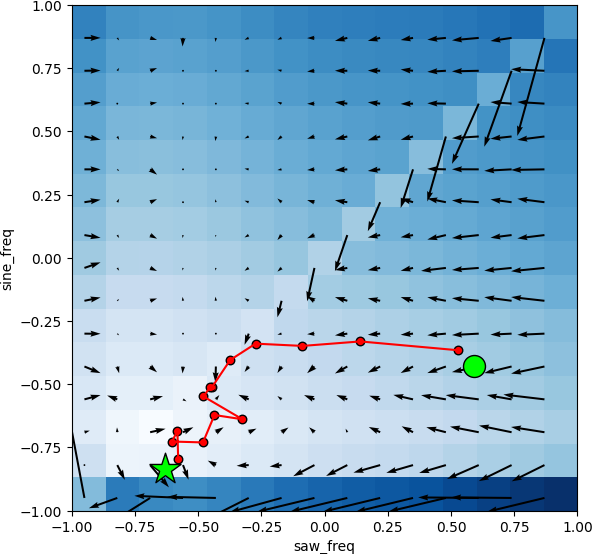
\includegraphics[width=\textwidth]{images/experiment_plots/p1_JTFS.png}}
        \caption{JTFS loss}
        \label{fig:p1_jtfs}
    \end{subfigure}

    \caption{Gradient descent fields for each loss with respect to \AddSineSaw{}. The initial and target parameters are shown with green circle \greencircle~and star \greenstar~respectively. High loss corresponds to dark-blue and low corresponds to white.}
    \label{fig:p1_losses}
\end{figure*}

\begin{figure*}[htbp]
    \centering
    % Top row
    \begin{subfigure}[b]{0.49\textwidth}
        \centering
        \adjustbox{valign=t}{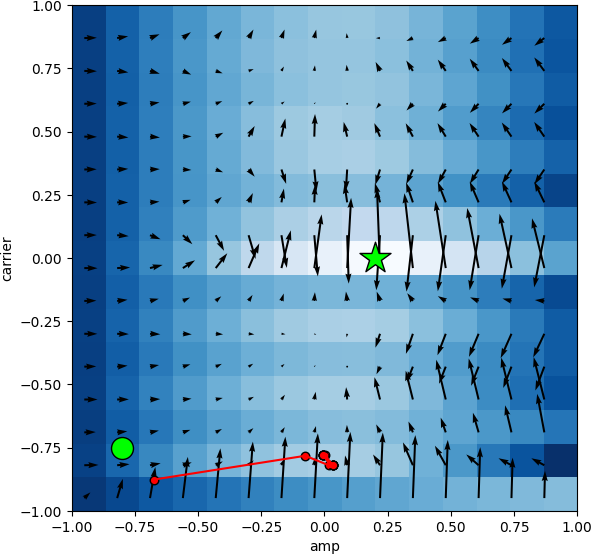
\includegraphics[width=\textwidth]{images/experiment_plots/p2_L1_Spec.png}}
        \caption{L1 spectrogram loss}
        \label{fig:p2_spec}
    \end{subfigure}
    \hfill
    \begin{subfigure}[b]{0.49\textwidth}
        \centering
        \adjustbox{valign=t}{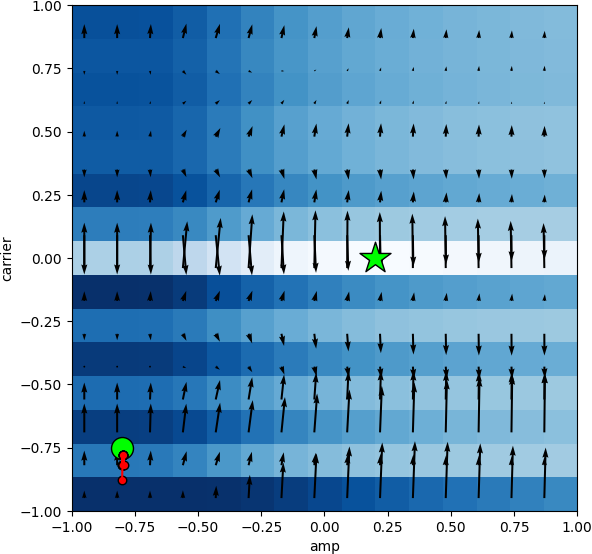
\includegraphics[width=\textwidth]{images/experiment_plots/p2_SIMSE_Spec.png}}
        \caption{SIMSE spectrogram loss}
        \label{fig:p2_simse}
    \end{subfigure}
    \vspace{0.5cm} 
    % Bottom row
    \begin{subfigure}[b]{0.49\textwidth}
        \centering
        \adjustbox{valign=t}{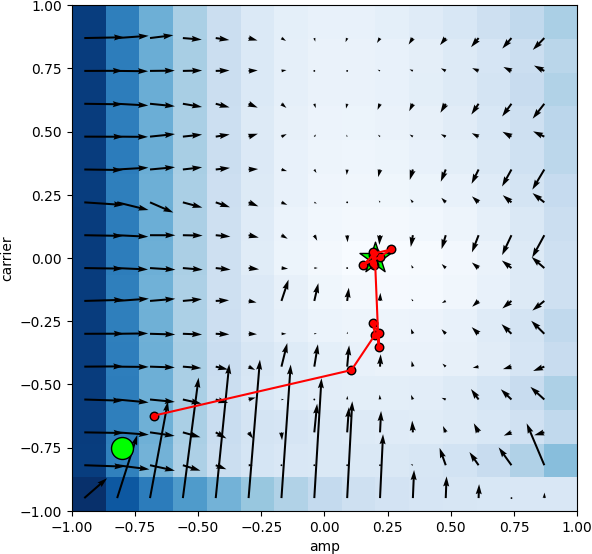
\includegraphics[width=\textwidth]{images/experiment_plots/p2_DTW_Onset.png}}
        \caption{DTW onset loss.}
        \label{fig:p2_dtw}
    \end{subfigure}
    \hfill
    \begin{subfigure}[b]{0.49\textwidth}
        \centering
        \adjustbox{valign=t}{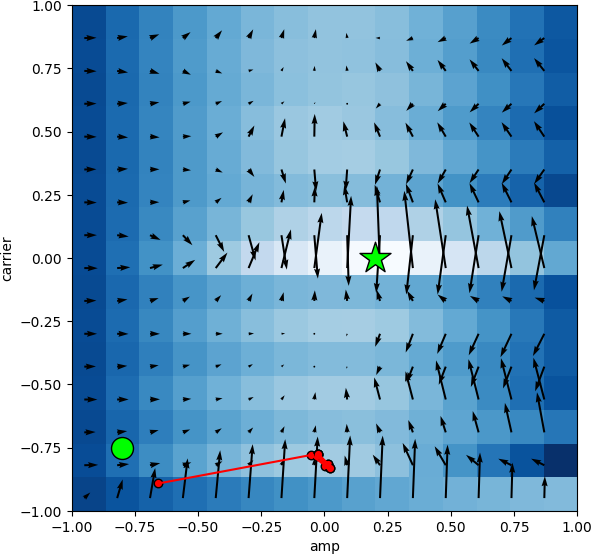
\includegraphics[width=\textwidth]{images/experiment_plots/p2_JTFS.png}}
        \caption{JTFS loss}
        \label{fig:p2_jtfs}
    \end{subfigure}

    \caption{Gradient descent fields for each loss with respect to \AmpMod. The initial and target parameters are shown with green circle \greencircle~and star \greenstar~respectively. High loss corresponds to dark-blue and low corresponds to white.}
    \label{fig:p2_losses}
\end{figure*}

\begin{figure*}[htbp]
    \centering
    % Top row
    \begin{subfigure}[b]{0.49\textwidth}
        \centering
        \adjustbox{valign=t}{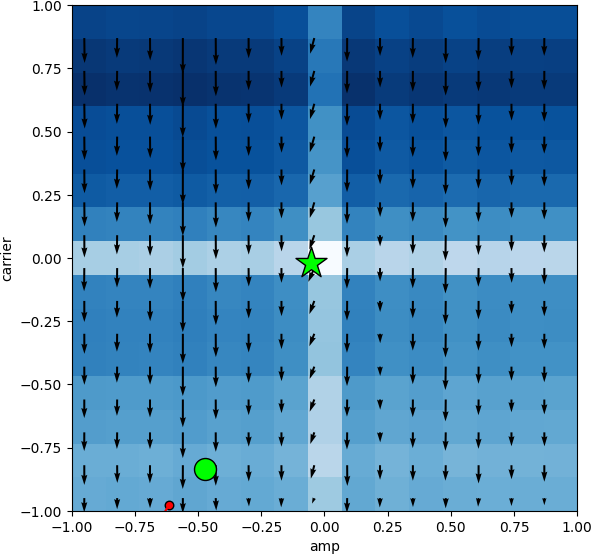
\includegraphics[width=\textwidth]{images/experiment_plots/p3_L1_Spec.png}}
        \caption{L1 spectrogram loss}
        \label{fig:p3_spec}
    \end{subfigure}
    \hfill
    \begin{subfigure}[b]{0.49\textwidth}
        \centering
        \adjustbox{valign=t}{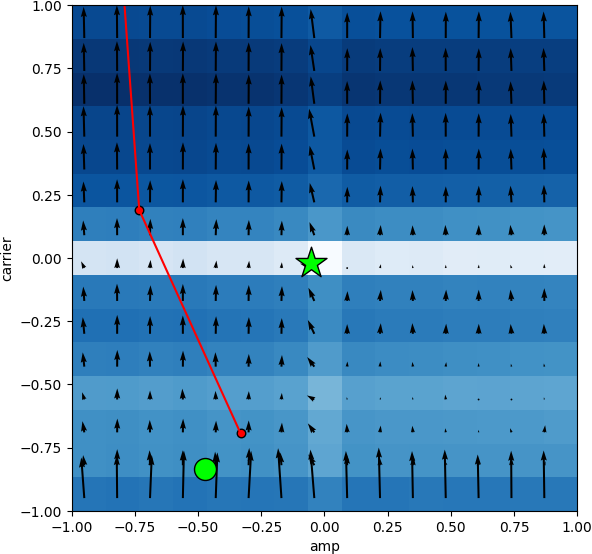
\includegraphics[width=\textwidth]{images/experiment_plots/p3_SIMSE_Spec.png}}
        \caption{SIMSE spectrogram loss}
        \label{fig:p3_simse}
    \end{subfigure}
    \vspace{0.5cm} 
    % Bottom row
    \begin{subfigure}[b]{0.49\textwidth}
        \centering
        \adjustbox{valign=t}{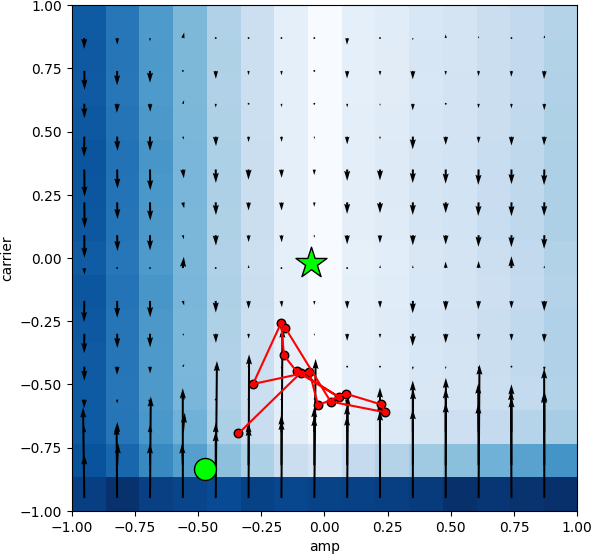
\includegraphics[width=\textwidth]{images/experiment_plots/p3_DTW_Onset.png}}
        \caption{DTW onset loss.}
        \label{fig:p3_dtw}
    \end{subfigure}
    \hfill
    \begin{subfigure}[b]{0.49\textwidth}
        \centering
        \adjustbox{valign=t}{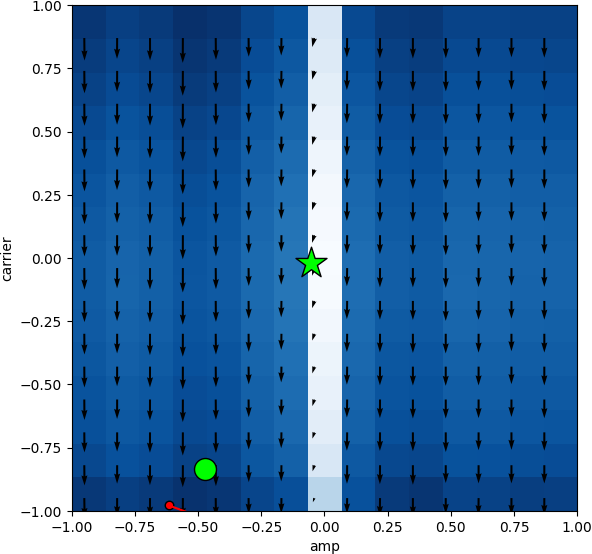
\includegraphics[width=\textwidth]{images/experiment_plots/p3_JTFS.png}}
        \caption{JTFS loss}
        \label{fig:p3_jtfs}
    \end{subfigure}

    \caption{Gradient descent fields for each loss with respect to \FMMod. The initial and target parameters are shown with green circle \greencircle~and star \greenstar~respectively. High loss corresponds to dark-blue and low corresponds to white.}
    \label{fig:p3_losses}
\end{figure*}

% \section{Appendix B}
% \label{appendix:parameters}
% List of arbitrary parameters used in this work.\\
% % name,  value
% % learning rate, 0.45
% % iterations, 200
% % number of experiments, 200
% % bootstrapping k, 1000
% % bootstrapping n, 50\% or 100
% % sample length, 1 sec
% % sample rate, 44100 (cite)
% \begin{verbatim}
% | Name                  | Value           |
% |-----------------------|-----------------|
% | Learning Rate         | 0.45            |
% | Iterations            | 200             |
% | Number of Experiments | 200             |
% | Bootstrapping k       | 1000            |
% | Bootstrapping n       | 50% or 100      |
% | Sample Length         | 1 sec           |
% | Sample Rate           | 44100 (cite)    |
% | DTW gamma             | 1               |
% \end{verbatim}


